
\section{Analiza systemu}

Celem projektu była analiza możliwości przetwarzania równoległego w architekturze czwórki z początkowymi danymi w dolnym węźle P1 (jak pokazano na rysunku \ref{fig:schema}).
W ramach projektu zajmowaliśmy się dwoma modelami - sekwencyjnym oraz równoległym z jedną komunikacją na łączu.

\begin{figure}[!ht]
\centering
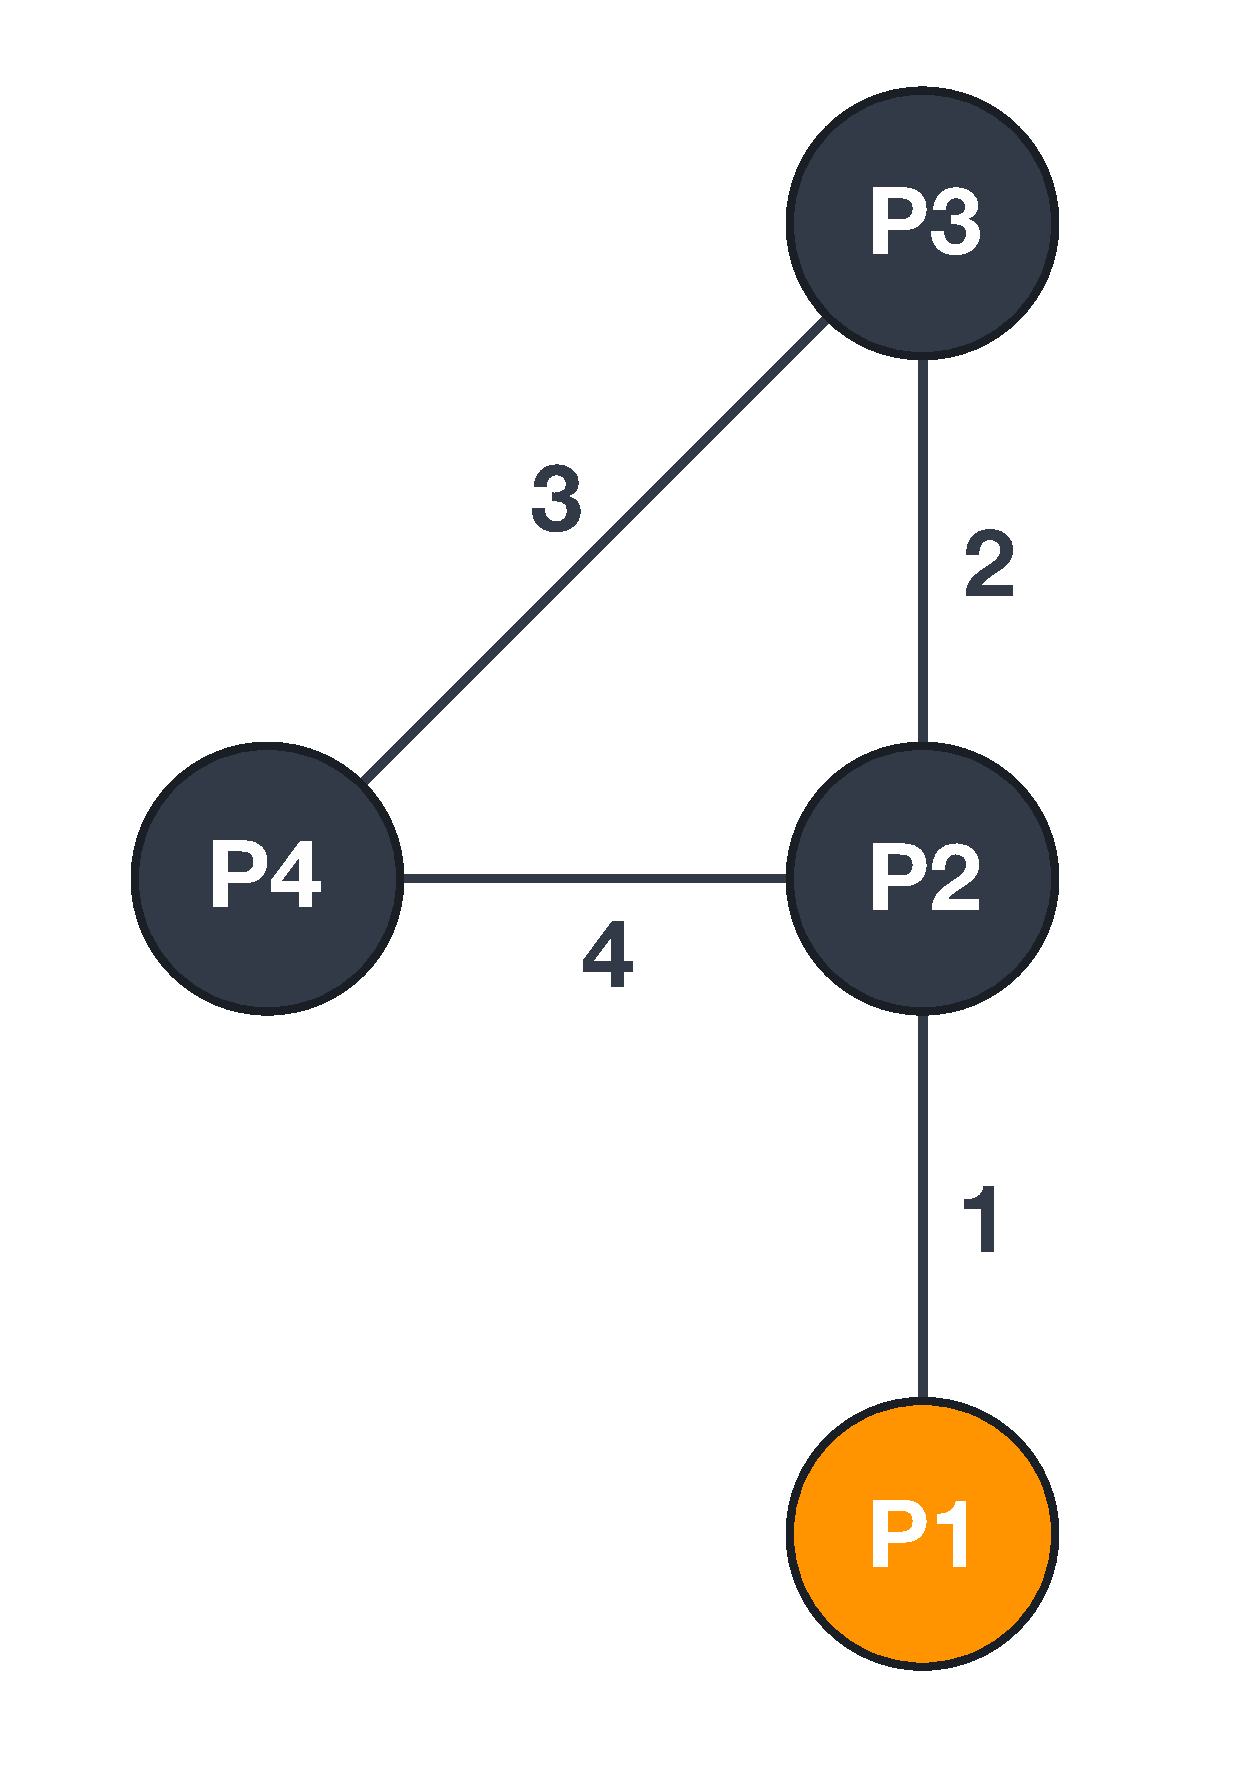
\includegraphics[width=0.5\textwidth]{schema.pdf}
\caption{Schemat systemu wraz z oznaczeniem procesorów}
\label{fig:schema}
\end{figure}

Biorąc pod uwagę fakt, że węzeł P1 jako jedyny  posiada dane w stanie początkowym może on odgrywać jedynie rolę nadawcy danych. Węzeł P2 może zarówno otrzymywać (z węzła P1), jak i nadawać dane (do węzłów P3 i P4). Na łączu 1 komunikacja będzie się odbywać w kierunku “do” węzła P2, natomiast na łączach 2 i 4 będzie się odbywać w kierunku “z” węzła P2. Niestety, nie możemy w modelu ogólnym założyć, czy dana komunikacja wystąpi. Trzeba pamiętać, że komunikacja na łączach 2 i 4 ma szanse wystąpić tylko jeśli wystąpi komunikacja na łączu 1 (węzeł P2 otrzyma dane z węzła P1). Komunikacja na łączu 1 (pomiędzy węzłami P1 i P2) nie musi wystąpić jeśli koszt transmisji danych na tym łączy będzie stosunkowo duży. W przypadku węzłów P3 i P4 warto zauważyć symetrię \ref{fig:symetry}. Węzły te mogą pełnić zarówno rolę odbiorcy jak i nadawcy.

\begin{figure}[!ht]
\centering
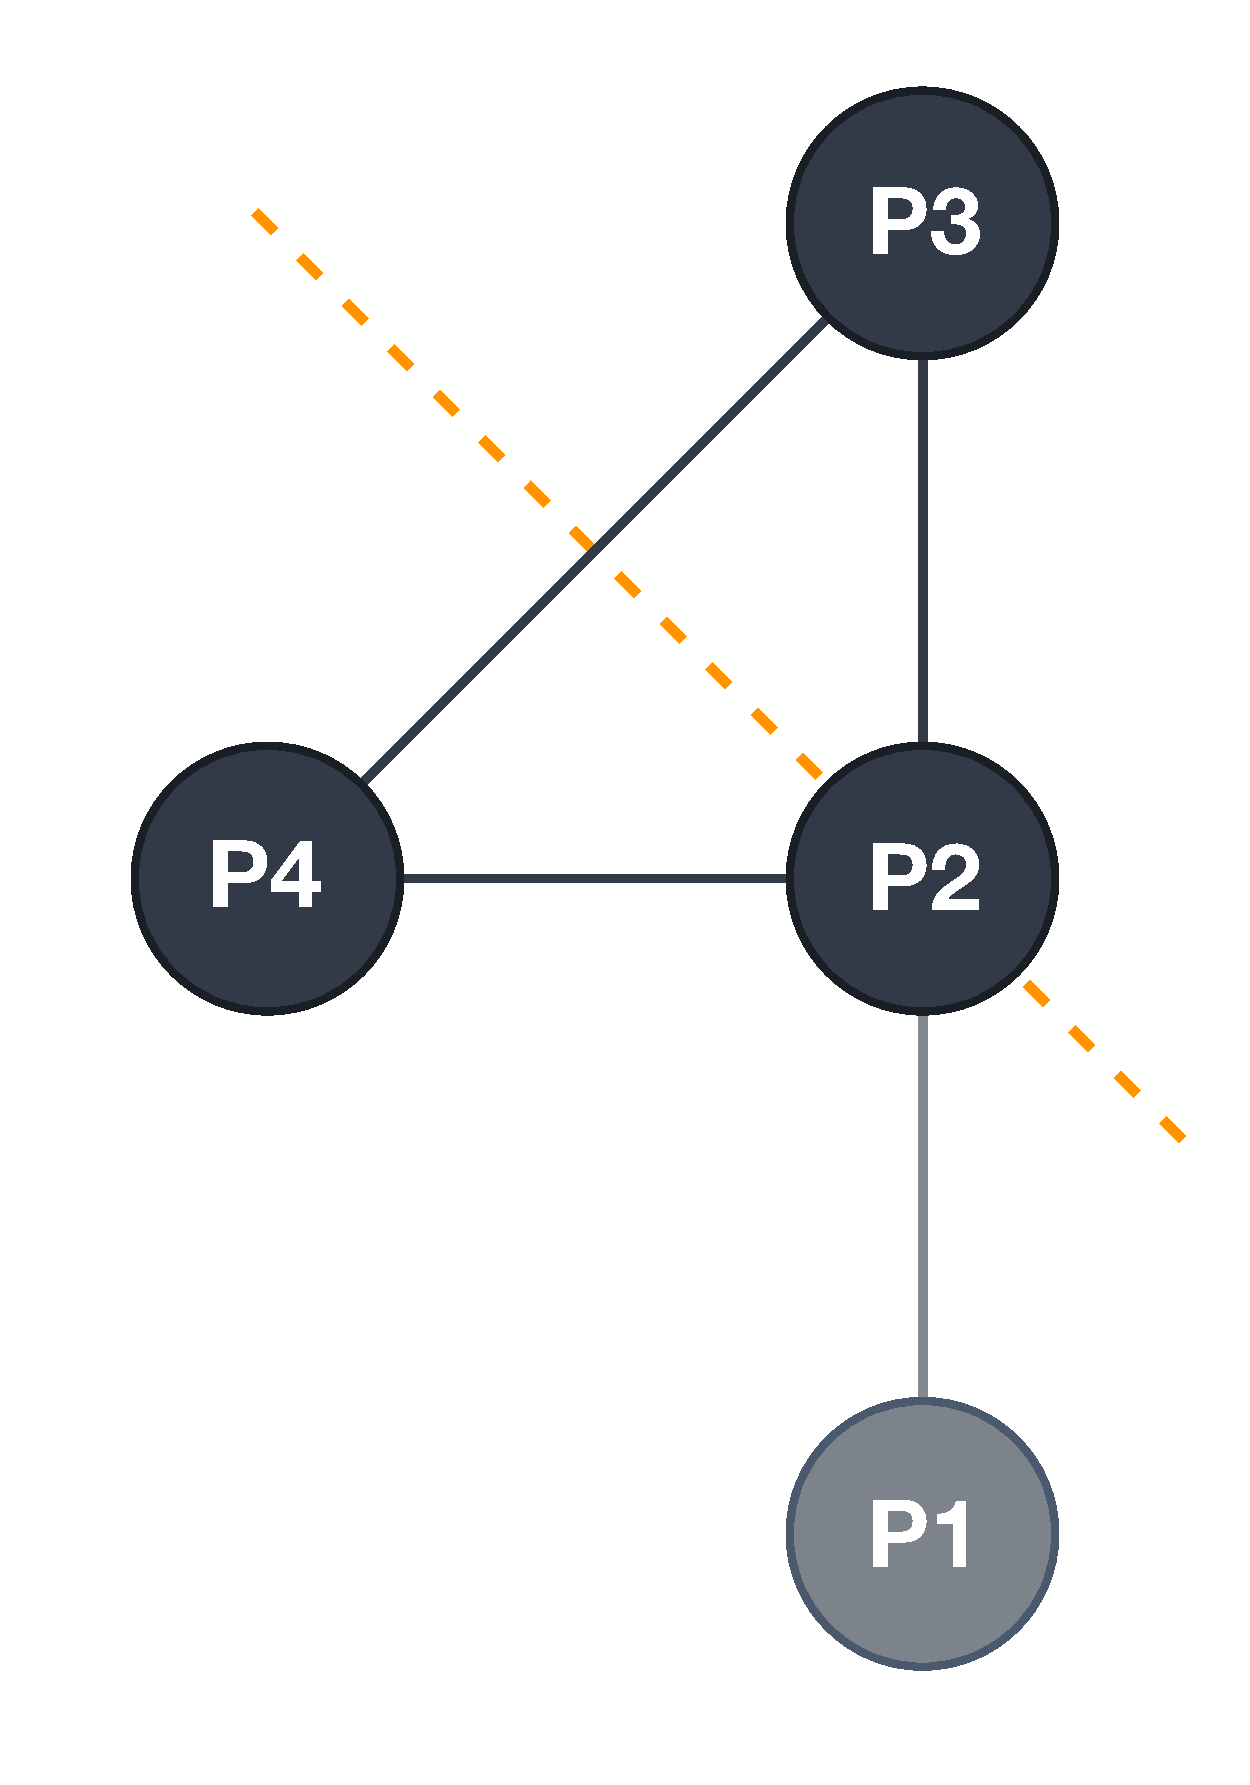
\includegraphics[width=0.5\textwidth]{symetry.pdf}
\caption{Symetria w analizowanym systemie (oznaczona linią przerywaną)}
\label{fig:symetry}
\end{figure}

W przypadku modeli sekwencyjnych transmisja pomiędzy urządzeniami może się odbyć tylko i wyłącznie gdy oba nie wykonują żadnych obliczeń i nie uczestniczą w innej komunikacji. W przypadku zrównoleglenia obliczeń dopuszczalna jest jednoczesna komunikacja danego procesora z więcej niż jednym urządzeniem oraz dokonywania obliczeń na danych znajdujących się na tymże procesorze. Zważając na fakt, że porcje danych są liczbami całkowitymi należy mieć na uwadze konieczność synchronizacji urządzeń.

Dla każdego z modeli minimalizowana jest wartość $T$, która jest większa bądź równa od wszystkich wartości $T_x$ (czas zakończenia wszystkich działań na procesorze $Px$) gdzie $x = 1, 2, 3, 4$.
 
\subsection{Analiza modelu sekwencyjnego}

Analiza modelu sekwencyjnego.

\subsubsection{Pierwszy model sekwencyjny}

\subsubsection{Drugi model sekwencyjny}

\subsubsection{Trzeci model sekwencyjny}

\subsection{Analiza modelu równoległego}

Analiza modelu równoległego.

\subsubsection{Pierwszy model równoległy}

\subsubsection{Drugi model równoległy}

